\documentclass[11pt,aspectratio=169]{beamer}
\usetheme{Boadilla}
\usecolortheme{beaver}
\usepackage[utf8]{inputenc}
\usepackage[spanish,mexico]{babel}
\usepackage{amsmath}
\usepackage{amsfonts}
\usepackage{amssymb}
\usepackage{graphicx}
\usepackage{booktabs}
\usepackage{listings}
\usepackage{multicol}
\usepackage{multirow}
\usepackage{algorithm,algorithmic}
\author{Héctor Selley}
\title{Máquinas de soporte vectorial}
\providecommand{\tightlist}{%
  \setlength{\itemsep}{0pt}\setlength{\parskip}{0pt}}
%\setbeamercovered{transparent} 
%\setbeamertemplate{navigation symbols}{} 
%\logo{} 
\institute{Universidad Anáhuac México} 
\date{\today} 
%\subject{} 
\begin{document}

\AtBeginSection[] % Do nothing for \section*
{
\begin{frame}<beamer>
\frametitle{Contenido}
\tableofcontents[currentsection]
\end{frame}
}

\begin{frame}
	\titlepage
\end{frame}

%\begin{frame}
%	\tableofcontents
%\end{frame}

\section{¿Qué son las máquinas de soporte vectorial?}
\begin{frame}{¿Qué son las SVM?}
  Las máquinas de soporte vectorial (SVM) son un conjunto de métodos de aprendizaje supervisado utilizados para: \pause
	\begin{itemize}\pause
		\item Clasificiación \pause
		\item Regresión\pause
		\item Detección de outliers
	\end{itemize}
\end{frame}

\begin{frame}{Ventajas de las SVM}
  Algunas ventajas de las máquinas de soporte vectorial son:\pause
  \begin{itemize}
    \item Muy efectivas en espacios de alta dimensión. \pause
    \item Efectivas en los casos donde el número de las dimensiones sea mayor que el número de muestras. \pause 
    \item Utiliza un subconjunto de puntos de entrenamiento en la función decisión (llamados soporte vectorial), 
      por lo que es eficiente en uso de memoria. \pause
    \item Versatilidad: Se pueden especificar diferentes \textit{funciones kernel} para la función de decisión. 
      Existe un conjunto de kernels común pero se puede utilizar uno personalizado.
  \end{itemize}
\end{frame}

\begin{frame}{Desventajas de las SVM}
  Algunas desventajas de las máquinas de soporte vectorial son:\pause
  \begin{itemize}
    \item Si el número de características es mucho mayor que el número de muestras, es crucial evitar un 
      sobreajuste al elegir las funciones kernel y el término de regularización. \pause
    \item SVM's no proporcionan directamente la estimación de probabilidad, éstas se calculan utilizando 
      una costosa validación cruzada de cinco pliegues.
  \end{itemize}
\end{frame}

\begin{frame}{¿Qué son las máquinas de soporte vectorial?}
  \begin{itemize}
    \item Las máquinas de soporte vectorial en \textit{scikit-learn} soportan como entrada el \textit{vector de muestra denso} 
      y el \textit{vector de muestra escaso}. \pause
    \item Sin embargo, para utilizar una SVM para realizar predicciones para un 
      conjunto de datos escasos, se debe realizar un ajuste a esos datos.\pause
    \item Para un desempeño óptimo, se debe utilizar una matriz C-ordered tipo \textit{numpy.ndarray} (denso) o 
      \textit{scipy.sparse.csr\_matrix} (escaso).
  \end{itemize}
\end{frame}

\section{Descripción General}
\begin{frame}{Descripción General}
	\begin{enumerate}
		\item \textbf{Selección del tipo de SVM}: Primero, debes decidir si utilizarás una SVM para clasificación o regresión. 
			Las SVM para clasificación se utilizan para separar las muestras en diferentes clases, mientras que las 
			SVM para regresión se utilizan para predecir valores continuos.\pause
		\item \textbf{Preprocesamiento de datos}: Prepara tus datos de entrenamiento y asegúrate de que estén en un formato 
			adecuado. Esto puede implicar la normalización, estandarización o cualquier otro tipo de procesamiento necesario 
			para garantizar una representación adecuada de las características.\pause
		\item \textbf{Selección de características}: Si tienes muchas características en tus datos, puedes utilizar técnicas de 
			selección o extracción de características para reducir su dimensión y mejorar el rendimiento del modelo SVM. 
	\end{enumerate}
\end{frame}

\begin{frame}{Descripción General}
	\begin{enumerate}
		\setcounter{enumi}{3}
		\item \textbf{Entrenamiento}: Durante la fase de entrenamiento, la SVM busca encontrar el hiperplano óptimo que mejor 
			separe las muestras de diferentes clases. Este hiperplano se elige de manera que maximice la distancia (margen) 
			entre las muestras de entrenamiento más cercanas de diferentes clases. Las muestras de entrenamiento más cercanas 
			al hiperplano se llaman vectores de soporte.\pause
		\item \textbf{Selección del kernel}: El kernel es una función que mapea los datos de entrada a un espacio de mayor 
			dimensionalidad donde es más fácil separar las clases. Los kernels comunes utilizados en SVM incluyen el lineal, 
			polinómico, radial basis function (RBF) y el sigmoidal. La elección del kernel depende de la naturaleza de los datos 
			y la complejidad del problema.
	\end{enumerate}
\end{frame}

\begin{frame}{Descripción General}
	\begin{enumerate}
		\setcounter{enumi}{5}
		\item \textbf{Ajuste de parámetros}: Las SVM tienen parámetros que deben ajustarse, como el parámetro de regularización 
			(C) y el parámetro del kernel. Estos parámetros afectan el equilibrio entre la clasificación correcta de los datos 
			de entrenamiento y la capacidad de generalización del modelo. Es importante ajustar estos parámetros mediante técnicas 
			de validación cruzada para obtener un modelo óptimo. \pause
		\item \textbf{Clasificación o predicción}: Una vez entrenado el modelo SVM, puedes utilizarlo para clasificar nuevos datos 
			en el caso de SVM para clasificación, o para predecir valores continuos en el caso de SVM para regresión. El modelo 
			asignará las nuevas muestras a una clase específica o proporcionará una estimación numérica según corresponda.
	\end{enumerate}
\end{frame}

\begin{frame}{Descripción General}
	\begin{itemize}
		\item Es importante destacar que las SVM son algoritmos muy potentes y versátiles \pause 
		\item pero también pueden requerir un ajuste cuidadoso de parámetros y un preprocesamiento adecuado de los datos 
			para obtener los mejores resultados.\pause 
		\item Además, pueden ser computacionalmente costosos en conjuntos de datos grandes.
	\end{itemize}
\end{frame}

\section{Clasificación}
\begin{frame}{Clasificación}
  Para llevar a cabo una clasificación se puede utilizar: \pause
  \begin{itemize}
    \item SVC \pause
    \item NuSVC \pause
    \item LinearSVC 
  \end{itemize}
\end{frame}

\begin{frame}{Clasificación}
\begin{description}
  \item[SVC: Clásificación de Vector de Soporte-C.]  El tiempo de ajuste escala al menos cuadráticamente con el número de muestras 
    y puede ser impráctico si se tienen decenas de miles de muestras.\pause 
  \item[NuSVC: Clasificación de Vector de Soporte-Nu.] Similar a SVC pero utiliza un parámetro para controlar el número de vectores de soporte. \pause
  \item[LinearSVC: Clasificación de Vector de Soporte Lineal.] Similar a SVC pero tiene mayor flexibilidad en la elección de funciones de 
    penalización y pérdida, por lo que debería escalar mejor para un conjunto muy grande de muestras.
\end{description} 
\end{frame}

\begin{frame}{Clasificación}
  Dichas clases realizan una clasificación binaria y multiclase en un conjunto de datos.\pause
  \begin{figure}
    \centering
    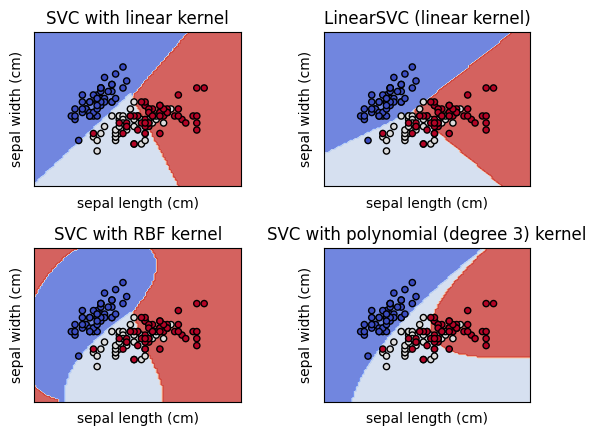
\includegraphics[scale=0.5]{ML/701.png}
  \end{figure}
\end{frame}

\begin{frame}{Clasificación}
  \begin{itemize}
    \item \textbf{SVC} y \textbf{NuSVC} son métodos similares pero aceptan conjuntos de parámetros ligeramente diferentes (diversos) y 
      tienen diferentes formulaciones matemáticas. \pause
    \item \textbf{LinearSVC} es una implementación más rápida de la clasificación de vector de soporte (SVC) con kernel lineal. \pause
    \item La función de decisión SVM depende de un subconjunto del conjunto de entrenamiento, llamado \textbf{vector de soporte}.
  \end{itemize}
\end{frame}

\section{Problemas desbalanceados}
\begin{frame}{Problemas desbalanceados}
  \begin{itemize}
    \item SVM puede dar más importancia a ciertas clases o a ciertas muestras individuales \pause
    \item Esto se llama peso de clase o peso de muestra. \pause
    \item La figura ilustra el perímetro de decisión de un problema desbalanceado, con y sin 
      corrección de peso.
  \end{itemize}
\end{frame}

\begin{frame}{Problemas desbalanceados}
  \begin{figure}
    \centering
    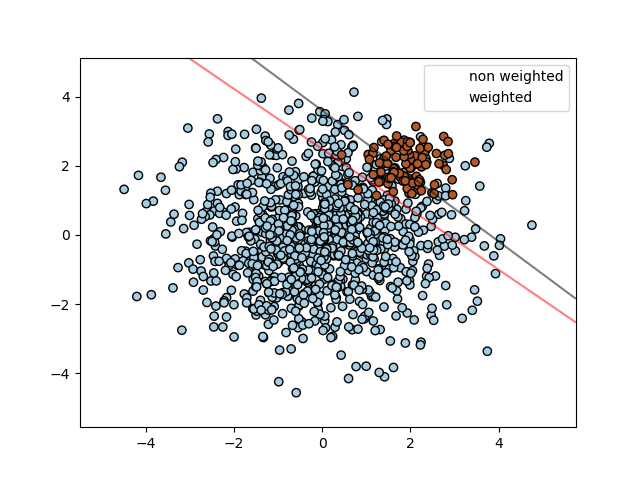
\includegraphics[scale=0.6]{img/701.png}
  \end{figure}
\end{frame}

\begin{frame}{Problemas desbalanceados}
  \begin{figure}
    \centering
    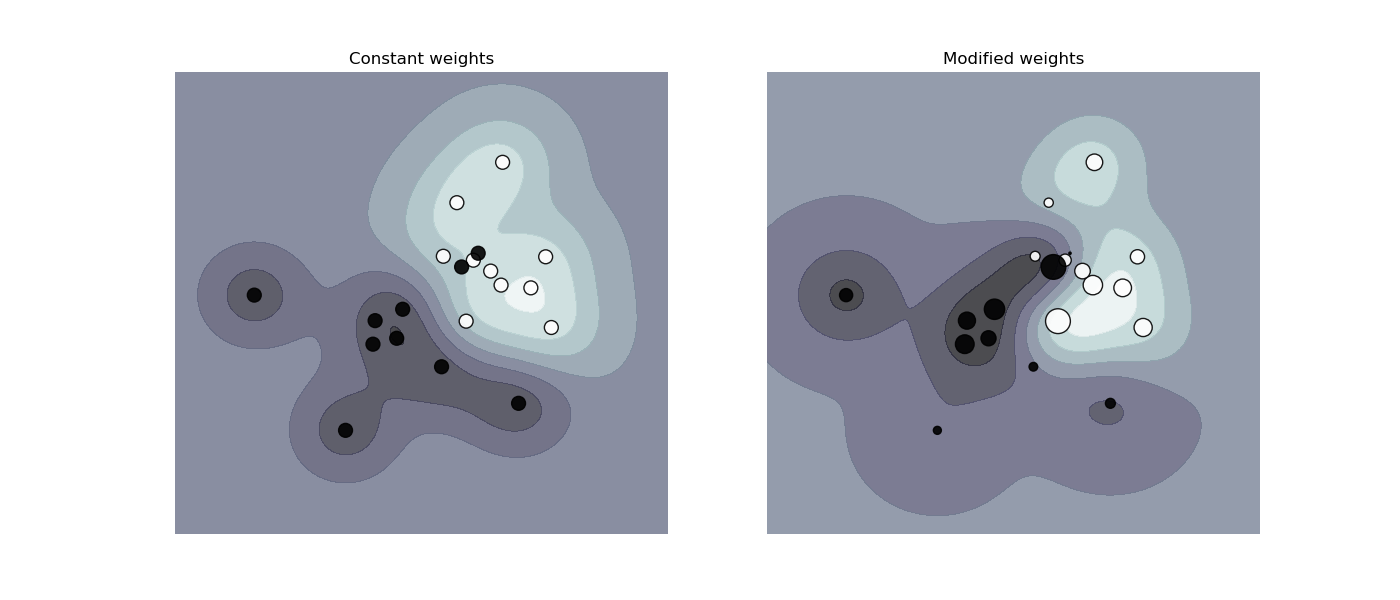
\includegraphics[scale=0.45]{img/702.png}
  \end{figure}
\end{frame}


\section{Regresión}
\begin{frame}{Regresión}
  \begin{itemize}
    \item El método de soporte vectorial puede extenderse para resolver problemas de regresión\pause: \textbf{Regresión de Vectores de Soporte}\pause
    \item El modelo producido por la clasificación de vectores de soporte depende únicamente de un subconjunto del conjunto de entrenamiento \pause
    \item Esto debido a que la función costo para la construcción del modelo no toma en cuenta puntos que se encuentran más allá del margen. 
  \end{itemize}
\end{frame}

\begin{frame}{Regresión}
  Existen tres diferentes implementaciones de la Regresión de Vectores de Soporte. \pause
  \begin{description}
    \item[SVR: Regresión de Vectores de Soporte-Epsilon] La complejidad del tiempo de ajuste es más que cuadrática con el número de muestras, 
      lo que dificulta escalar a conjuntos de datos con más de un par de 10000 muestras. \pause
    \item[NuSVR: Regresión de Vectores de Soporte-Nu] Similar a NuSVC, para la regresión, usa un parámetro nu para controlar la cantidad de vectores de soporte. Sin embargo, 
      a diferencia de NuSVC, donde nu reemplaza a C, aquí nu reemplaza el parámetro epsilon de epsilon-SVR.\pause
    \item[LinearSVR: Regresión de Vectores de Soporte Lineal] Similar a SVR con el parámetro kernel='linear', tiene más flexibilidad en la elección de penalizaciones y funciones de 
      pérdida y debería escalar mejor a un gran número de muestras.
  \end{description}
\end{frame}

\begin{frame}{Regresión}
  \begin{itemize}
    \item LinearSVR es más rápido que SVR pero solo considera el caso lineal \pause 
    \item NuSVR implementa una formulación matemática ligeramente diferente que SVR y LinearSVR.
  \end{itemize}
\end{frame}


\section{Funciones kernel}
\begin{frame}{Funciones kernel}
  Las funciones kernel más comúnes son las siguientes:\pause
  \begin{itemize}
    \item Lineal \pause
    \item Polinomial \pause
    \item RBF (Función de Base Radial)\pause
    \item Sigmoide
  \end{itemize}
\end{frame}

\begin{frame}{BRF}
	\begin{itemize}
		\item Cuando se entrena un SVM con kernel SBF se deben considerar dos parámetros: $C$ y $gamma$. \pause
		\item $C$ compensa la clasificación errónea de las muestras de entrenamiento contra la simplicidad 
			de la superficie de decisión\pause
		\item Un valor bajo de $C$ suaviza la superficie de decisión, mientras que un valor alto de $C$ pretende clasificar 
			correctamente todos los ejemplos de entrenamiento.\pause
		\item $gamma$ define cuánta influencia tiene una sola muestra de entrenamiento.\pause
		\item Cuanto mayor sea $gamma$, más cerca deben estar otras muestras para verse afectadas.
	\end{itemize}
\end{frame}

\section{Bibliografía}
\begin{frame}[allowframebreaks]{References}
    \nocite{*}
    \bibliographystyle{plain}
    \bibliography{biblioSVM}
\end{frame}

\end{document}
